\subsection{U-Net}\label{s:unet}
\chapterauthor{Woon Jun Wei (2200624)}

The U-Net architecture, introduced by Ronneberger et al. in 2015, is a pioneering model for biomedical image segmentation, widely adopted for various image segmentation tasks \cite{ronneberger_u-net_2015}. U-Net features a symmetric architecture with a contracting path to capture context and an expansive path for precise localization. The architecture includes skip connections that concatenate feature maps from the contracting path to the expanding path, enhancing the segmentation performance (see Figure \ref{f:unet}).

\begin{figure}[H] 
	\centering
	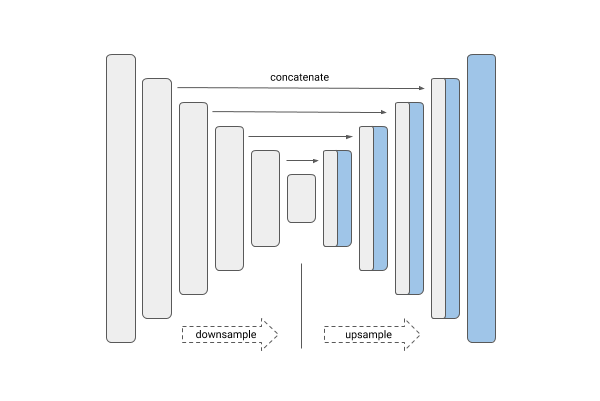
\includegraphics[width=0.5\textwidth]{unet/unet.png}
	\caption{Simple U-Net architecture}\label{f:unet}
\end{figure}

\subsubsection{Implementation}

U-Net++, an extension introduced by Zhou et al. in 2018, improves the original architecture by incorporating dense skip connections. These connections concatenate feature maps from all previous layers in the contracting path to the expanding path, enhancing feature reuse and segmentation accuracy \cite{zhou_unet_2018}.

Due to the complexity and time constraints associated with training, evaluation, and tuning, a U-Net model was not architected from scratch. Instead, this study employed the U-Net++ architecture using the \texttt{segmentation\_models} library \cite{Yakubovskiy_2019}. This library offers implementations of various deep learning models for image segmentation, supporting pre-trained models such as VGG, ResNet, and EfficientNet as down-sampling backbones.

Input images were preprocessed by cropping, enhancing, and resizing to $224 \times 224 \times 3$, as detailed in Section \ref{image_cropping_enhancement}. Further preprocessing included normalization, horizontal flipping, and random rotation by 20 degrees, managed by the \texttt{ImageDataGenerator} class, which also handled the 80:20 training-validation split.

The implemented model architecture was U-Net++ with an EfficientNetB1 backbone, initialized with ImageNet weights. To obtain classification results for the full image instead of pixel-wise classification, a Global Average Pooling layer followed by a Dense layer with four units and a softmax activation function was added. The model was compiled using the categorical cross-entropy loss function and accuracy metric.

Training was conducted using the Adam optimizer with a learning rate of 0.0001 and a batch size of 10 for 100 epochs. The best model was saved based on validation loss, incorporating Checkpointing, Early Stopping, and Reduce Learning Rate on Plateau. Training halted at 33 epochs due to early stopping, achieving a validation loss of 0.1862 and a validation accuracy of 0.9444.

\subsubsection{Results and Evaluation}

\begin{figure}[H]
  \begin{center}
    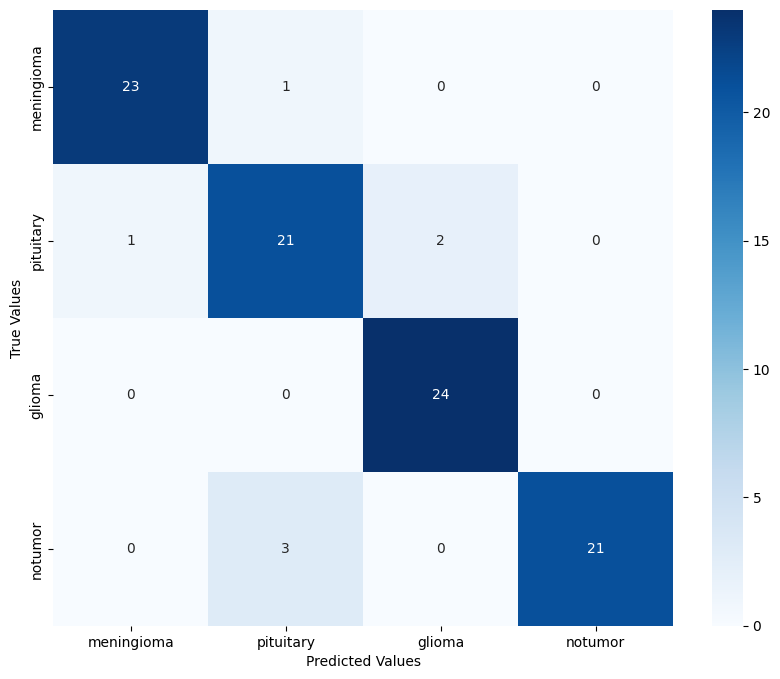
\includegraphics[width=0.35\textwidth]{unet/evaluation/cm1.png}
    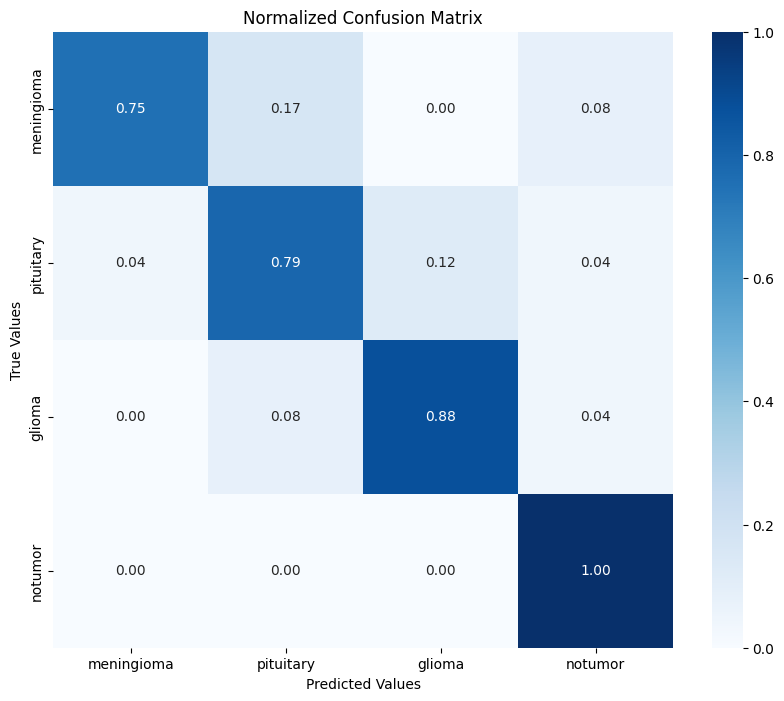
\includegraphics[width=0.35\textwidth]{unet/evaluation/cm2.png}
    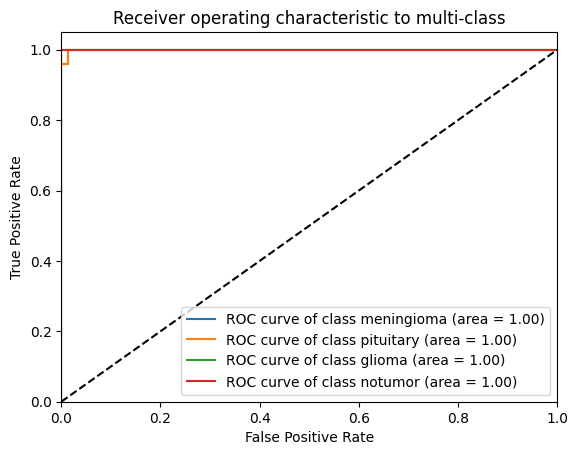
\includegraphics[width=0.35\textwidth]{unet/evaluation/ROC.png}
    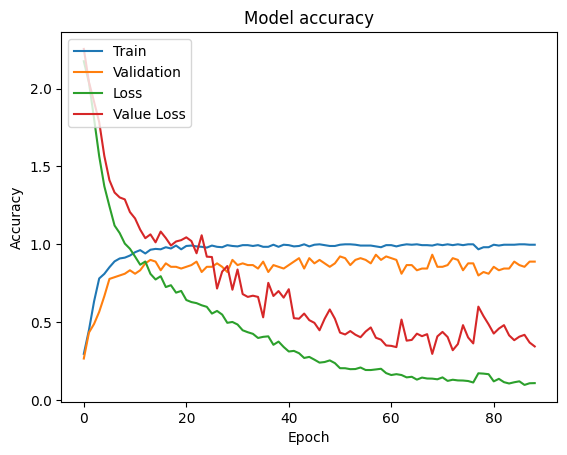
\includegraphics[width=0.35\textwidth]{unet/evaluation/learning_curve.png}
  \end{center}
  \caption{Confusion Matrix, ROC Curve, and Learning Curve for Brain Tumor Segmentation}\label{f:unet_evaluation}
\end{figure}

\begin{longtable}{|l|c|c|c|c|}
\caption{Classification Report for Brain Tumor Segmentation} \label{tab:unet_classification_report}
\hline \textbf{Class} & \textbf{Precision} & \textbf{Recall} & \textbf{F1-Score} & \textbf{Support} \\ \hline 
\endfirsthead

\multicolumn{5}{c}%
{{\bfseries \tablename\ \thetable{} -- continued from previous page}} \\
\hline \textbf{Class} & \textbf{Precision} & \textbf{Recall} & \textbf{F1-Score} & \textbf{Support} \\ \hline 
\endhead

\hline \multicolumn{5}{|r|}{{Continued on next page}} \\ \hline
\endfoot

\hline
\endlastfoot

meningioma & 0.96 & 0.92 & 0.94 & 24 \\ 
\hline
pituitary  & 0.91 & 0.88 & 0.89 & 24 \\ 
\hline
glioma     & 0.92 & 1.00 & 0.96 & 24 \\ 
\hline
notumor    & 0.96 & 0.96 & 0.96 & 24 \\ 
\hline
micro avg  & 0.94 & 0.94 & 0.94 & 96 \\ 
\hline
macro avg  & 0.94 & 0.94 & 0.94 & 96 \\ 
\hline
weighted avg & 0.94 & 0.94 & 0.94 & 96 \\ 
\hline
samples avg & 0.94 & 0.94 & 0.94 & 96 \\ 
\end{longtable}

\begin{longtable}{|c|c|c|c|}
\caption{Additional Metrics for Brain Tumor Segmentation} \label{tab:unet_additional_metrics}
\hline \textbf{DSC} & \textbf{Sensitivity} & \textbf{Specificity} & \textbf{Accuracy} \\ 
\hline
\endfirsthead

\multicolumn{4}{c}%
{{\bfseries \tablename\ \thetable{} -- continued from previous page}} \\
\hline \textbf{DSC} & \textbf{Sensitivity} & \textbf{Specificity} & \textbf{Accuracy} \\ \hline
\endhead

\hline \multicolumn{4}{|r|}{{Continued on next page}} \\ \hline
\endfoot

\hline
\endlastfoot

0.9370 & 0.9375 & 0.9792 & 0.9375 \\ \hline
\end{longtable}

The performance metrics presented in Tables \ref{tab:unet_classification_report} and \ref{tab:unet_additional_metrics} demonstrate the robust capability of the U-Net model in brain tumor segmentation. The classification report (Table \ref{tab:unet_classification_report}) highlights the model's high precision, recall, and F1-scores across all classes, with an overall accuracy of 0.94. Specifically, the model achieved precision scores of 0.96, 0.91, 0.92, and 0.96 for the meningioma, pituitary, glioma, and notumor classes, respectively. Corresponding recall values were 0.92, 0.88, 1.00, and 0.96, indicating the model's effectiveness in identifying true positives for each class.

The confusion matrix in Figure \ref{f:unet_evaluation} (top-left) provides a visual representation of the model's classification accuracy, revealing a minimal number of misclassifications. The ROC Curve (bottom left) further substantiates the model's excellent performance, demonstrating a strong ability to distinguish between different classes.

Additional evaluation metrics in Table \ref{tab:unet_additional_metrics} confirm the model's robustness. The Dice Similarity Coefficient (DSC) of 0.9370 indicates a high overlap between the predicted and actual tumor regions, underscoring the model's precise segmentation capabilities. Sensitivity and specificity values of 0.9375 and 0.9792, respectively, further highlight the model's accuracy in detecting tumor presence while minimizing false positives.

Mentioned in \cite{abd-ellah_automatic_2024}, the varying nature and size of glioma tumors pose significant challenges for accurate segmentation. Despite these challenges, the U-Net model achieved an impressive F1-score of 0.96 for glioma, indicating a low incidence of false positives and false negatives. This performance suggests that the model is highly effective in segmenting glioma tumors, although there remains potential for further improvement. Fine-tuning the model or employing additional data augmentation techniques could enhance the segmentation accuracy for glioma tumors, thereby improving overall model performance.

% In conclusion, the U-Net model exhibits strong performance in brain tumor segmentation, as evidenced by the high precision, recall, F1-scores, and additional metrics. The results indicate a high degree of accuracy and reliability, making the U-Net model a valuable tool for medical image analysis and diagnostic applications.


% The metrics in Tables \ref{tab:unet_classification_report} and \ref{tab:unet_additional_metrics} demonstrate the U-Net model's strong performance in brain tumor segmentation. The model achieved high precision, recall, and F1-scores across all classes, with an overall accuracy of 0.9444. The confusion matrix in Figure \ref{f:unet_evaluation} (top-left) further illustrates the model's ability to accurately classify brain tumor images. The ROC Curve (Bottom Left) demonstrates the model's excellent performance in distinguishing between classes. Additionally, the high DSC, sensitivity, and specificity values in Table \ref{tab:unet_additional_metrics} confirm the model's robustness in segmenting brain tumors.
% 
% Mentioned in \cite{abd-ellah_automatic_2024}, the varying nature and size of the glioma tumor makes it difficult to segment accurately. However, the U-Net model achieved a high F1-score of 0.96 for glioma, where little false positives and false negatives were observed. This suggests that the model may benefit from further fine-tuning to improve segmentation accuracy for glioma tumors or additional data augmentation to enhance generalization.


